% BHU PYQ -- Professional Exam Template
\documentclass[11pt,a4paper]{article}

\usepackage[a4paper,top=2.5cm,bottom=2.5cm,left=2.8cm,right=2.8cm,headheight=14pt]{geometry}
\usepackage{amsmath,amssymb}
\usepackage[T1]{fontenc}
\usepackage[utf8]{inputenc}
\usepackage{lmodern}
\usepackage{microtype}
\usepackage{fancyhdr}
\usepackage{enumitem}
\usepackage{hyperref}
\usepackage{lastpage}
\usepackage{parskip}
\usepackage{tikz}
\usetikzlibrary{arrows.meta,shapes,positioning}

\hypersetup{colorlinks=true,urlcolor=black,linkcolor=black,
  pdftitle={B.Sc. (Hons.) Zoology Sem-V ZOB-501 -- BHU PYQ}}

\pagestyle{fancy}
\fancyhf{}
\renewcommand{\headrulewidth}{0.4pt}
\renewcommand{\footrulewidth}{0.4pt}
\fancyhead[L]{\small   \textit{Banaras Hindu University}}
\fancyhead[R]{\small   \textit{Zoology Paper: ZOB-501}}
\fancyfoot[C]{\small Page  \thepage\ of \pageref{LastPage}}


\newlist{parts}{enumerate}{2}
\setlist[parts,1]{label=(\alph*),leftmargin=*,itemsep=4pt,topsep=3pt}
\setlist[parts,2]{label=(\roman*),leftmargin=*,itemsep=2pt,topsep=2pt}

\newcommand{\pts}[1]{\hfill   \textit{[#1]}}


\begin{document}


\begin{center}
  {\large\bfseries BANARAS HINDU UNIVERSITY}\\[2pt]
  {
\normalsize B.Sc. (Hons.) Semester V Examination, 2022-23}\\[6pt]
  \rule{0.8\linewidth}{0.5pt}\\[6pt]
  {\large\bfseries Zoology}\\[4pt]
  {\large\bfseries Paper: ZOB-501 --- Functional Anatomy of Nonchordates}\\[4pt]
  {
\normalsize Time: Three hours \hfill Full Marks: 70}
\end{center}

\rule{\linewidth}{0.4pt}

\smallskip



\noindent   \textit{Note: Answer six questions including Question No. 1 which is compulsory. Draw diagrams wherever necessary. The figures in the right-hand margin indicate marks.}

\bigskip




\noindent   \textbf{Question 1.} Answer the following parts:

\begin{parts}
  \item Define the following terms:\pts{$4  \times 1 = 4$}
  
\begin{parts}
    \item Laurer's canal
    \item Hexacanth
    \item Medusa
    \item Rhopalia.
  \end{parts}
  
  \item State whether the following statements are True or False. Give brief justification for your answer:\pts{$4  \times 2 = 8$}
  
\begin{parts}
    \item Polypoid phase is dominant phase in   \textit{Aurelia}.
    \item In   \textit{Fasciola} the germ cells of Cercaria gives rise to Metacercaria.
    \item Genital papilla is only found in male   \textit{Ascaris}.
    \item Coelom in   \textit{Unio} is schizocoelic.
  \end{parts}

  \item Differentiate between the following:\pts{$4  \times 2 = 8$}
  
\begin{parts}
    \item Hydrozoa and Scyphozoa
    \item Canal system and Water vascular system
    \item Nereis and Heteronereis
    \item Protonephridia and Nephridia.
  \end{parts}
\end{parts}

\medskip


\noindent   \textbf{Question 2.} With the help of neat labeled diagrams, explain different types of canal system in sponges.\pts{10}


\begin{center}

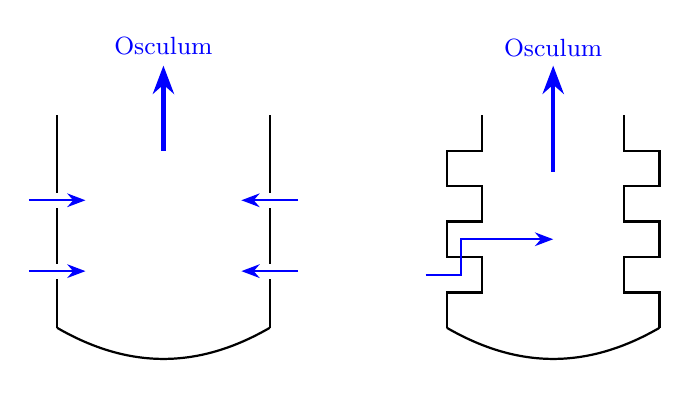
\begin{tikzpicture}[scale=0.9, >=Stealth, every node/.style={font=\small}]
  
\begin{scope}[shift={(0,0)}]
    
ode[above] at (1.5, 3.2) {   \textbf{Asconoid Canal System}};
    % Outer wall
    \draw[thick] (0,0) -- (0,3);
    \draw[thick] (3,0) -- (3,3);
    \draw[thick] (0,0) to[out=-30, in=210] (3,0);
    
    % Ostia
    \foreach \y in {0.8, 1.8} {
      \draw[fill=white, draw=white] (-0.1,\y-0.1) rectangle (0.1,\y+0.1);
      \draw[fill=white, draw=white] (2.9,\y-0.1) rectangle (3.1,\y+0.1);
      \draw[->, thick, blue] (-0.4, \y) -- (0.4, \y);
      \draw[->, thick, blue] (3.4, \y) -- (2.6, \y);
    }
    
ode[left, blue] at (-0.4, 1.3) {Ostium};
    
    % Spongocoel
    
ode at (1.5, 1.3) {Spongocoel};
    
    % Osculum
    \draw[->, ultra thick, blue] (1.5, 2.5) -- (1.5, 3.7) node[above] {Osculum};
  \end{scope}

  
\begin{scope}[shift={(5.5,0)}]
    
ode[above] at (1.5, 3.2) {   \textbf{Syconoid Canal System}};
    % Folded walls
    \draw[thick] (0,0) -- (0,0.5) -- (0.5,0.5) -- (0.5,1.0) -- (0,1.0) -- (0,1.5) -- (0.5,1.5) -- (0.5,2.0) -- (0,2.0) -- (0,2.5) -- (0.5,2.5) -- (0.5,3.0);
    \draw[thick] (3,0) -- (3,0.5) -- (2.5,0.5) -- (2.5,1.0) -- (3,1.0) -- (3,1.5) -- (2.5,1.5) -- (2.5,2.0) -- (3,2.0) -- (3,2.5) -- (2.5,2.5) -- (2.5,3.0);
    \draw[thick] (0,0) to[out=-30, in=210] (3,0);
    
    % Water path
    \draw[->, thick, blue] (-0.3, 0.75) -- (0.2, 0.75) -- (0.2, 1.25) -- (1.5, 1.25);
    
ode[font=\scriptsize, left] at (-0.3, 0.75) {Incurrent};
    
ode[font=\scriptsize, right] at (0.2, 1.25) {Radial};
    
    % Center spongocoel and osculum
    
ode at (1.5, 0.3) {Spongocoel};
    \draw[->, ultra thick, blue] (1.5, 2.2) -- (1.5, 3.7) node[above] {Osculum};
  \end{scope}
\end{tikzpicture}
\end{center}

\medskip


\noindent   \textbf{Question 3.} Describe the various larval forms of   \textit{Fasciola}.\pts{10}

\pagebreak

\medskip


\noindent   \textbf{Question 4.} Illustrate the life history of   \textit{Ascaris}. Add a note on its pathogenicity.\pts{10}

\medskip


\noindent   \textbf{Question 5.} Describe the structure of   \textit{Euglena} with a neat diagram. Comment on euglenoid movement.\pts{10}


\begin{center}

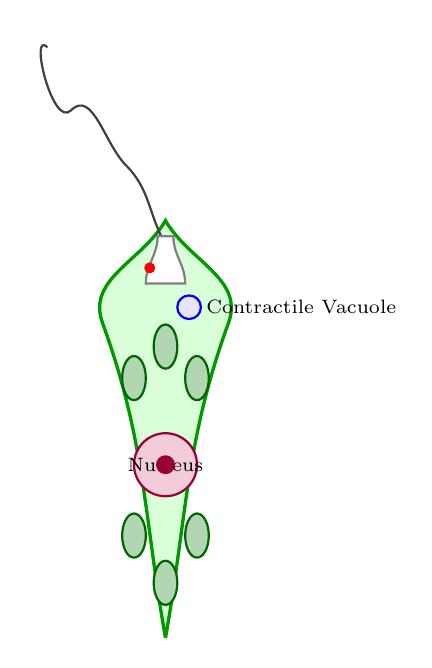
\begin{tikzpicture}[scale=1.0, >=Stealth, every node/.style={font=\small}]
  % Body
  \draw[fill=green!15, draw=green!60!black, very thick] 
    (0,-2.5) to[out=80, in=-110] (0.8, 1.5) to[out=70, in=-60] (0, 2.8)
    to[out=240, in=110] (-0.8, 1.5) to[out=-70, in=100] (0,-2.5);
  
  % Flagellum
  \draw[thick, darkgray] (0, 2.5) to[out=120, in=-45] (-0.5, 3.5) to[out=135, in=45] (-1.2, 4.2) to[out=225, in=135] (-1.5, 5.0);
  
ode[left] at (-1.5, 5.0) {Flagellum};
  
  % Reservoir
  \draw[fill=white, draw=gray, thick] (-0.25, 2.0) to[out=90, in=-90] (-0.1, 2.6) -- (0.1, 2.6) to[out=-90, in=90] (0.25, 2.0) -- cycle;
  
ode[right, font=\scriptsize] at (0.25, 2.3) {Reservoir};
  
  % Stigma
  \fill[red] (-0.2, 2.2) circle (2pt);
  
ode[left, red, font=\scriptsize] at (-0.2, 2.2) {Stigma};
  
  % Contractile vacuole
  \draw[circle, fill=blue!10, draw=blue, thick] (0.3, 1.7) circle (0.15) node[right=0.1cm, font=\scriptsize, black] {Contractile Vacuole};
  
  % Nucleus
  \draw[fill=purple!20, draw=purple!80!black, thick] (0, -0.3) circle (0.4) node[font=\scriptsize, align=center] {Nucleus};
  \fill[purple!80!black] (0, -0.3) circle (0.12);
  
  % Chloroplasts
  \foreach \pos in {(-0.4, 0.8), (0.4, 0.8), (-0.4, -1.2), (0.4, -1.2), (0, 1.2), (0, -1.8)} {
    \draw[fill=green!45!black!30, draw=green!40!black, thick] \pos ellipse (0.15 and 0.28);
  }
  
ode[right, green!40!black, font=\scriptsize] at (0.45, 0.8) {Chloroplast};
  
  
ode[below=0.2cm] at (0, -2.5) {   \textbf{Structure of }   \textit{Euglena viridis}};
\end{tikzpicture}
\end{center}

\medskip


\noindent   \textbf{Question 6.} Give a detailed account of male and female reproductive system of   \textit{Palaemon}.\pts{10}

\medskip


\noindent   \textbf{Question 7.} Describe water vascular system of starfish and mention the role of this system in its life.\pts{10}

\pagebreak

\medskip


\noindent   \textbf{Question 8.} Write short notes on any two of the following:\pts{$2  \times 5 = 10$}

\begin{parts}
  \item Parasitic adaptations in   \textit{Taenia}
  \item Trochophore larva
  
  
\begin{center}
  
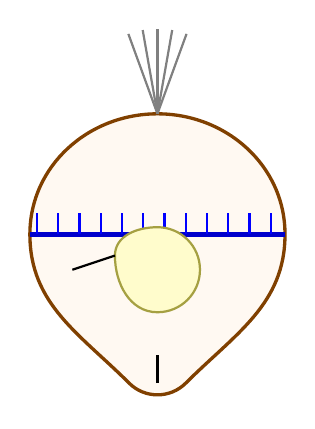
\begin{tikzpicture}[scale=0.9, >=Stealth, every node/.style={font=\small}]
    % Pear-shaped body
    \draw[fill=orange!5, draw=orange!50!black, very thick] 
      (0, 2) to[out=0, in=90] (1.8, 0.3) to[out=-90, in=45] (0.4, -1.8)
      to[out=225, in=-45] (-0.4, -1.8) to[out=135, in=-90] (-1.8, 0.3) to[out=90, in=180] (0, 2) -- cycle;
    
    % Apical tuft
    \foreach \angle in {70, 80, 90, 100, 110} {
      \draw[thick, gray] (0, 2) -- ({1.2*cos(\angle)}, {2 + 1.2*sin(\angle)});
    }
    
ode[above=0.6cm] at (0, 2) {Apical Tuft};
    
    % Prototroch
    \draw[ultra thick, blue!80!black] (-1.8, 0.3) -- (1.8, 0.3);
    \foreach \x in {-1.7, -1.4, -1.1, -0.8, -0.5, -0.2, 0.1, 0.4, 0.7, 1.0, 1.3, 1.6} {
      \draw[thick, blue] (\x, 0.3) -- (\x, 0.6);
    }
    
ode[right, blue!80!black] at (1.8, 0.45) {Prototroch};
    
    % Gut
    \draw[fill=yellow!20, draw=yellow!60!black, thick] (-0.6, 0) to[out=-90, in=180] (0, -0.8) to[out=0, in=-90] (0.6, -0.2) to[out=90, in=0] (0, 0.4) to[out=180, in=90] (-0.6, 0);
    
ode[font=\scriptsize] at (0, -0.2) {Stomach};
    
    % Mouth
    \draw[thick] (-1.2, -0.2) -- (-0.6, 0);
    
ode[left, font=\scriptsize] at (-1.2, -0.2) {Mouth};
    
    % Anus
    \draw[thick] (0, -1.8) -- (0, -1.4);
    
ode[below, font=\scriptsize] at (0, -1.8) {Anus};
  \end{tikzpicture}
  \end{center}

  \item Torsion.
\end{parts}

\vfill
\rule{\linewidth}{0.4pt}

\begin{center}\small
\href{https://bhu-exam.vercel.app/}{Click Here}\\[4pt]\href{https://me-aryan.vercel.app/}{Click Here}\\[4pt]\href{https://quashan-me.vercel.app/}{Click Here}
\end{center}

\end{document}
